\documentclass[xcolor=x11names, aspectratio=169]{beamer}
\usepackage[ngerman]{babel}
\usepackage{amsmath}
\usepackage{amssymb}
\usepackage{amsfonts}
\usepackage{mathpazo}
\usepackage{enumerate}
\usepackage{array,booktabs}
\usepackage{tikz}
\usepackage[version=4,arrows=pgf-filled]{mhchem}
\usepackage{mathdots}
\usepackage{multirow}
\usepackage{tabularx}
\usetikzlibrary{matrix,backgrounds,patterns,arrows,decorations.markings,shapes}
\usepackage{caption}

\usetheme[titleformat title=regular,titleformat frame=regular,titleformat section=allcaps,numbering=fraction]{metropolis}

\mhchemoptions{mathfontcommand=\mathsf}

\author[Felix Kußmaul]{\large Felix Kußmaul}
\title[NAA]{\Large Die Neutronenaktivierungsanalyse}
\subtitle{Einführung und Anwendungen in der Archäologie}
\institute[UzK]{Seminar zu naturwissenschaftlichen Untersuchungsmethoden\\ von Fundkeramik und ihrer archäologischen Interpretation\\[.5em] Universität zu Köln}
\date[23.\ Juli 2016]{23.\ Juli 2016}

\newcommand{\red}[1]{\textcolor{red}{#1}}
\newcommand{\orange}[1]{\textcolor{orange}{#1}}
\newcommand{\green}[1]{\textcolor{markgreen}{#1}}
\newcommand{\textgreen}[1]{\textcolor{textgreen}{#1}}
\newcommand{\blue}[1]{\textcolor{textblue}{#1}}
\newcommand{\gray}[1]{\textcolor{gray}{#1}}

\newcolumntype{R}{>{\centering\raggedleft\arraybackslash}X}
\newcolumntype{L}{>{\centering\raggedright\arraybackslash}X}
\newcolumntype{C}{>{\centering\arraybackslash}X}

\usepackage[firstinits=true,style=archaeologie,width=2cm,edby,backend=biber]{biblatex}
\addbibresource{naa.bib}
\renewcommand*{\bibfont}{\small}

\setbeamercovered{invisible}

\newcommand{\textsb}[1]{{\fontfamily{cmss}\fontseries{sbc}\fontshape{n}\selectfont #1}}

\setbeamertemplate{footline}
{
\hbox{%
  \begin{beamercolorbox}[wd=.28\paperwidth,ht=2.7ex,dp=1.2ex,center]{author in head/foot}%
    \usebeamerfont{author in head/foot}\insertshortauthor\ (\insertshortinstitute)
  \end{beamercolorbox}%
  \begin{beamercolorbox}[wd=.44\paperwidth,ht=2.7ex,dp=1.2ex,center]{author in head/foot}%
    \usebeamerfont{title in head/foot}\insertshorttitle:\ \textbf{\insertsection}
  \end{beamercolorbox}%
  \begin{beamercolorbox}[wd=.28\paperwidth,ht=2.7ex,dp=1.2ex,center]{author in head/foot}%
    \usebeamerfont{date in head/foot}\insertshortdate\hfill\insertframenumber/\inserttotalframenumber\strut
  \end{beamercolorbox}}
  \vskip0pt%
}

\tikzset{
  invisible/.style={opacity=0},
  visible on/.style={alt={#1{}{invisible}}},
  alt/.code args={<#1>#2#3}{%
    \alt<#1>{\pgfkeysalso{#2}}{\pgfkeysalso{#3}} % \pgfkeysalso doesn't change the path
  },
}

\newcommand{\printSectionYes}{\AtBeginSubsection[]
{
 \begin{frame}{Agenda}
 \tableofcontents[sectionstyle=show/shaded,
 					subsectionstyle=show/shaded/hide]
 \end{frame}
}}

\tikzset{onslide/.code args={<#1>#2}{%
  \only<#1>{\pgfkeysalso{#2}}%
}}

\setbeamertemplate{section in toc shaded}[default][50]

\setbeamertemplate{subsection in toc shaded}[default][50]

\makeatletter
\patchcmd{\beamer@sectionintoc}{\vskip1.5em}{\vskip0.5em}{}{}
\makeatother

\makeatletter
\newcommand\footnoteref[1]{\protected@xdef\@thefnmark{\ref{#1}}\@footnotemark}
\makeatother

\setbeamertemplate{bibliography item}{%
  \ifboolexpr{ test {\ifentrytype{book}} or test {\ifentrytype{mvbook}}
    or test {\ifentrytype{collection}} or test {\ifentrytype{mvcollection}}
    or test {\ifentrytype{reference}} or test {\ifentrytype{mvreference}} }
    {\setbeamertemplate{bibliography item}[book]}
    {\ifentrytype{online}
       {\setbeamertemplate{bibliography item}[online]}
       {\setbeamertemplate{bibliography item}[article]}}%
  \usebeamertemplate{bibliography item}}
  
\defbibenvironment{bibliography}
  {\list{}
     {\settowidth{\labelwidth}{\usebeamertemplate{bibliography item}}%
      \setlength{\leftmargin}{\labelwidth}%
      \setlength{\labelsep}{\biblabelsep}%
      \addtolength{\leftmargin}{\labelsep}%
      \setlength{\itemsep}{\bibitemsep}%
      \setlength{\parsep}{\bibparsep}}}
  {\endlist}
  {\item}
\pgfdeclareimage[width=\columnwidth]{snucleus}{img/snucleus.eps}
\definecolor{morange}{HTML}{FF8200}
 
\begin{document}

\maketitle

\begin{frame}[<+->]{Before we start \dots}
\textbf{AGB:}
\begin{itemize}
\item Zu langsam/schnell/undeutlich? \textbf{Bitte meckern!}
\item Fragen \alert{jederzeit} willkommen
\item Du sollst keine anderen Editoren neben \texttt{vim} haben
\item \LaTeX\ $\gg$ MS Word, PowerPoint, \dots
\item Han shot first
\end{itemize}
\end{frame}

\begin{frame}{Agenda}
       \tableofcontents[ 
  		subsectionstyle=show, 
   	 	sectionstyle=show, 
   	 ] 
\end{frame}

\section{Einordnung}%\printSectionYes

\begin{frame}{Sinn und Zweck}
\begin{quote}
``NAA is a sensitive analytical technique useful for performing both qualitative and quantitative \alert{multi-element analysis} of major, minor, and trace elements in samples from almost every conceivable field of scientific or technical interest.''
\end{quote}
\vspace*{-2em}
\begin{flushright}
-- Dr.\ Michael Glascock, MURR
\end{flushright}
\end{frame}

\begin{frame}{\dots\ in der Archäologie}
\textbf{Wir Archäologen nutzen NAA seit Jahrzehnten erfolgreich für}
\begin{itemize}
\item die Bestimmung der \alert{Herkunft} eines Objektes
\item die Überprüfung der \alert{Echtheit} eines fragwürdigen Gegenstandes
\item Studien zur \alert{Herstellung} und \alert{Nutzung} von Artefakten
\end{itemize}
\end{frame}

\begin{frame}{Herkunftsbestimmung}
\textbf{Wir treffen folgende wichtige Annahmen:}
\begin{enumerate}[(i)]
\item Kein Handel mit Rohton
\item Bei hoher Präzision gilt ein Elementmuster als \alert{charakteristisch} für einen Ort
\item Gefäße mit gleichem Elementmuster stammen vom selben Ort
\item Das Muster veränderte sich nicht über die Zeit
\end{enumerate}
\end{frame}

\begin{frame}{Herkunftsbestimmung}
\begin{center}\Large
\begin{tabularx}{.9\columnwidth}{rlCrl}
\multirow{2}{*}{\parbox[c]{4.5em}{
\includegraphics[scale=.6]{img/pot.png}}}&&&&\multirow{2}{*}{\parbox[c]{4.5em}{
\includegraphics[scale=.6]{img/pot.png}}}\\
&\vphantom{$\overset{?}{=}$}\only<2-3>{Herkunft$_A$&$\overset{?}{=}$&Herkunft$_B$}&\\
&\onslide<3>{Muster$_A$&$=$&Muster$_B$}&\\
\end{tabularx}
\end{center}
\end{frame}
\begin{frame}{Herkunftsbestimmung}
\begin{center}\Large
\begin{tabularx}{.9\columnwidth}{rlCrl}
\multirow{2}{*}{\parbox[c]{4.5em}{
\includegraphics[scale=.6]{img/pot.png}}}&&&&\multirow{2}{*}{\parbox[c]{4.5em}{
\includegraphics[scale=.6]{img/pot.png}}}\\
&\color{morange}\vphantom{$\overset{?}{=}$}Herkunft$_A$&\color{morange}\vspace*{-1em}$=$&\color{morange}Herkunft$_B$&\\
&Muster$_A$&$=$&Muster$_B$&\\
\end{tabularx}
\end{center}
\end{frame}

\begin{frame}{Herkunftsbestimmung}
\textbf{Bekannte Herausforderungen:}
\begin{itemize}[<+->]
\item Nur selten wurde \alert{Rohton} direkt verwendet.

\textit{Meist wurde er vor dem Töpfern gesäubert oder mit anderem Ton vermischt.}
\item Variation bei der Aufbereitung führt zur \alert{Veränderung der Zusammensetzung}.

\textit{Es bedarf einer bekannten Referenzprobe.}
\item Veränderungen durch \alert{Brand und Bodenlagerung} für bestimmte Elemente.

\textit{Die betroffenen Elemente werden bei der Messung nicht berücksichtigt.}
\item Messungenauigkeiten oder -fehler.
\end{itemize}
\end{frame}

\begin{frame}{Herkunftsbestimmung}
\textbf{Problem mit Streuungen}

Gewisse Streuungen (5--10\,\%) sind \alert{normal} für Proben mit homogener Masse.

Zur Einteilung in Gruppen von Proben wollen wir nicht mehr als diesen Toleranzbereich zulassen, da sonst das \alert{zu \glqq diffuse\grqq\ Gesamtmuster} eine Unterscheidung verschiedener Herkünfte stark erschwert.
\end{frame}

\begin{frame}{Zuordnung: Muster $\mapsto$ Werkstatt}
\begin{itemize}
\item \textbf{Schwerster Schritt.}
\item \textbf{Notwendig:} Finden von Referenzmaterial \textit{für jede Produktionsserie}.

Dafür gut geeignet sind \alert{Fehlbrände} aus Abfallhaufen.\medskip\pause

\textit{Alternativ:} Logische Schlüsse anhand von \alert{Verteilungen}:

Lokale Produktion genau dann, wenn chemisches Muster dort in großen Stückzahlen gefunden wurde (nicht nur Keramik)
\end{itemize}
\end{frame}

\section{Methode}

\subsection{Probenherstellung}

\begin{frame}{Schritt 1: Probenentnahme}
\begin{minipage}{0.56\textwidth}\flushleft
\textbf{Entnahme der Probe vom Fundstück:}\smallskip

\begin{itemize}
\item mit Schaber o.\ Spitzbohrer

$\Rightarrow$ chemisch rein, z.\,B.\ synth.\ Saphir
\item z.\,B.\ vom Boden der Keramik
\item Bohrtiefe 1--2\,mm
\item 80\,mg \alert{Bohrstaub}
\item \glqq nicht zerstörerisch\grqq
\end{itemize}
\end{minipage}\hfill
\begin{minipage}{0.4\textwidth}
\begin{figure}
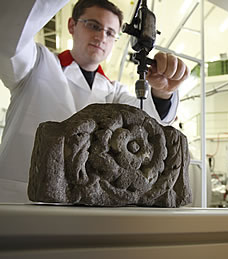
\includegraphics[width=.8\textwidth]{img/drill.jpg}
\caption{Entnahme der Probe, TRIGA Mainz.}
\end{figure}
\end{minipage}
\end{frame}

\begin{frame}{Schritt 2: Probenaufbereitung}
\begin{minipage}{0.5\textwidth}
\begin{figure}
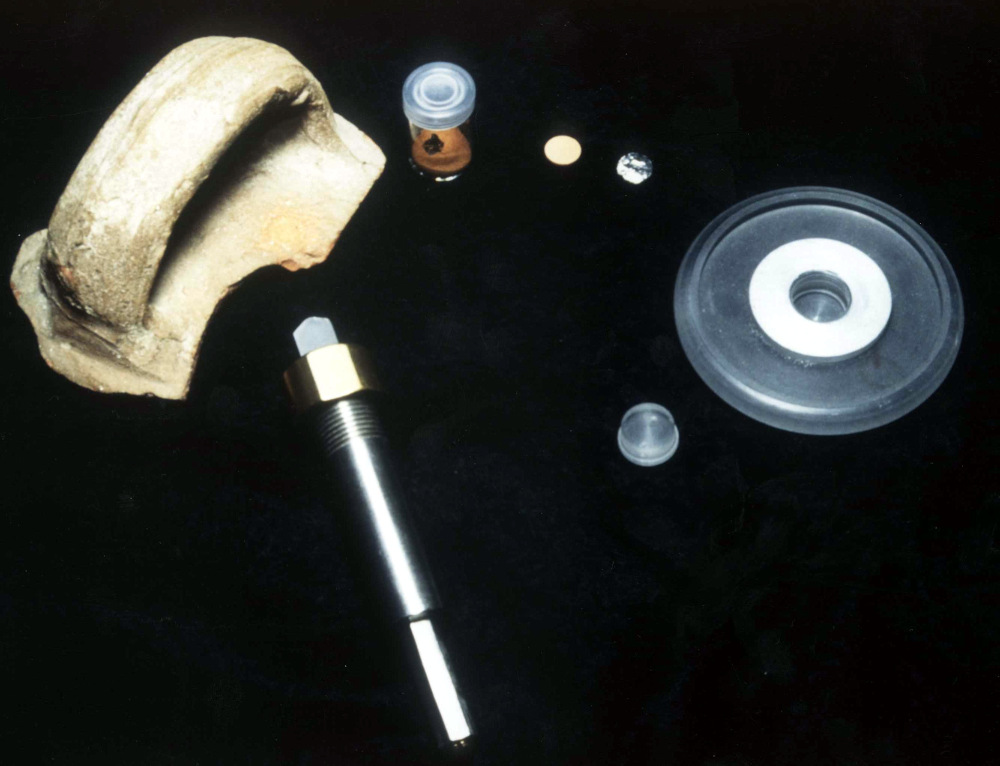
\includegraphics[width=\textwidth]{img/pill.jpg}
\caption{Objekt mit Bohrer, Tablette und Probenhalter, Mommsen 2002.}
\end{figure}
\end{minipage}\hfill
\begin{minipage}{.44\textwidth}\flushleft
\textbf{Bohrstaub wird zur Probe:}\smallskip

\begin{itemize}
\item chemisch reines Bindemittel, z.\,B.\ Zellulose
\item Herstellung einer \alert{Tablette}
\item Durchmesser von 10\,mm und Dicke von 1\,mm
\item Feste Abmessungen wichtig für genaue Messung des $\gamma$-Spektrums!
\end{itemize}
\end{minipage}
\end{frame}

\subsection{Neutronenbestrahlung}

\begin{frame}{Schritt 3: Neutronenbestrahlung}
\begin{minipage}{0.52\textwidth}\flushleft
Als Neutronenquelle werden häufig \textbf{Kernreaktoren} benutzt.\smallskip

\begin{itemize}
\item Spaltung von Uranisotopen\\$\Rightarrow$ therm.\ Neutronen mit $0,025$\,eV
\item $10^{12}$ bis $10^{14}$ Neutronen pro Sekunde und cm$^2$
\item Ein Durchgang für mehrere Proben gleichzeitig
\item \alert{Referenztablette} mit bekannter Zusammensetzung
\end{itemize}
\end{minipage}\hfill
\begin{minipage}{0.44\textwidth}
\begin{figure}
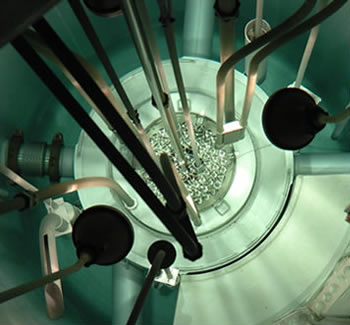
\includegraphics[width=\textwidth]{img/reactor-mainz.png}
\caption{TRIGA Reaktor, Mainz.}
\end{figure}
\end{minipage}
\end{frame}

\begin{frame}{Schritt 3: Neutronenbestrahlung}
\begin{figure}
\begin{minipage}{0.48\textwidth}
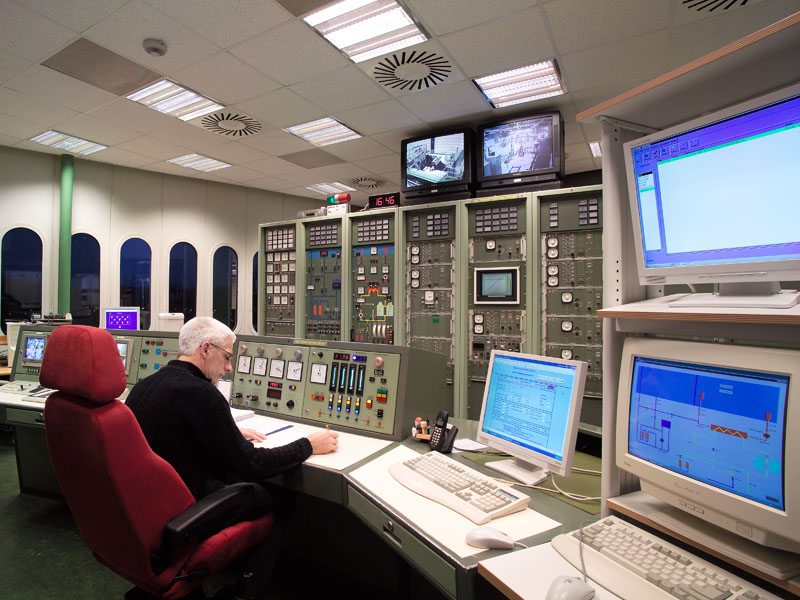
\includegraphics[width=\textwidth]{img/control-1.jpg}
\end{minipage}\hfill
\begin{minipage}{0.48\textwidth}
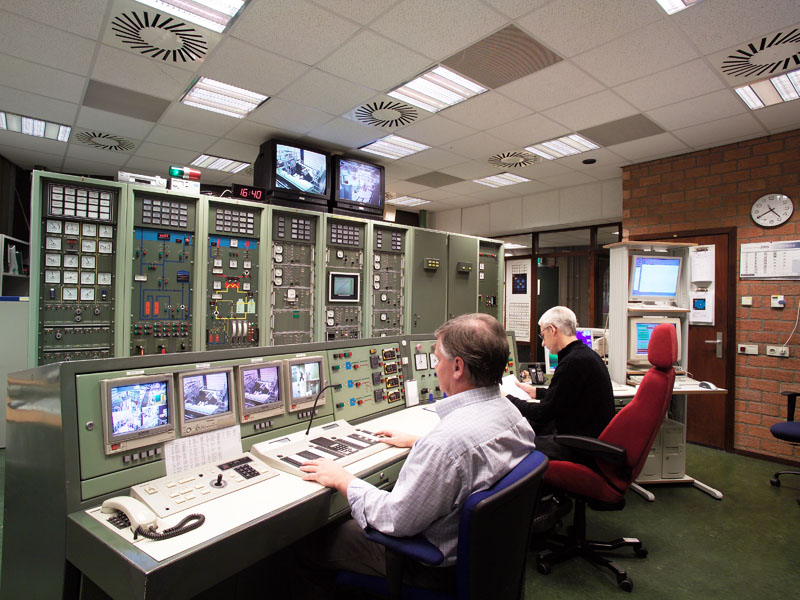
\includegraphics[width=\textwidth]{img/control-2.jpg}
\end{minipage}
\caption{Delft University of Technology, Kontrollraum.}
\end{figure}\vspace*{-1em}
\begin{center}
\href{run:/home/felix/naa.asf}{VIDEO!}
\end{center}
\end{frame}

\begin{frame}{Einschub: Grundbegriffe Kernphysik}
\begin{enumerate}[(i)]
\item \alert{Protonen} $p$ sind positiv geladene Teilchen mit Masse 1
\item \alert{Neutronen} $n$ sind el.\ neutral geladene Teilchen mit Masse 1
\item Protonen und Neutronen fassen wir als \alert{Nukleonen} zusammen\pause
\item Protonenzahl (\alert{Ordnungszahl}) $Z$ im Atomkern bestimmt das \emph{Element}
\item Nukleonenzahl (\alert{Massenzahl}) $A$ im Atomkern bestimmt die \emph{Atommasse}\pause
\item Wir schreiben für Element X: \[\text{\ce{^A_Z X}\quad oder kurz \quad\ce{^A X}}\]\pause\vspace*{-1.5em}
\item \alert{Isotopen} sind Elemente mit unterschiedlicher Masse
\item \alert{Halbwertszeit} $T_{1/2}$: Zeit, bis Hälfte des radioaktiven Stoffs zerfallen
\end{enumerate}
\end{frame}

\begin{frame}{Neutronenaktivierung}
\begin{center}\vspace*{-2.5em}
\begin{tikzpicture}
\draw[color=white,line width=.01pt] (-7,-3) grid[xstep=7cm, ystep=3cm] (7,3);

\pgfbox[center,center]{\pgfuseimage{snucleus}};

\node at (-6.4,-1.1) {$n$};
\node at (-5.2,-3.5) {\Large \ce{^{A}_{Z} X}};
\node at (-2.3,-3.5) {\Large \ce{^{A+1}_{Z} X^*}};
\node at (.4,-3.5) {\Large \ce{^{A+1}_{Z} X}};
\node at (3.2,-3.5) {\Large \ce{^{A+1}_{Z±1} Y^*}};
\node at (6.1,-3.5) {\Large \ce{^{A+1}_{Z±1} Y}};
\node at (2.5,2) {\large $\beta^\pm$};
\node at (-0.7,-1.6) {\Large $\gamma$};
\node at (4.9,-1.6) {\Large $\gamma$};
\end{tikzpicture}
\end{center}
\end{frame}

\begin{frame}{Neutronenaktivierung: Beispiel}
\begin{figure}
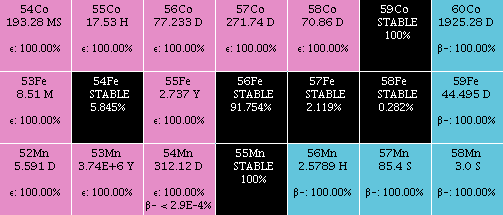
\includegraphics[height=.45\textheight]{img/nuclidchart.png}
\caption{Ausschnitt der Nuklidkarte.}
\end{figure}
\vspace*{-1em}
\[\large\text{\ce{^{58} Fe \:(n,$\gamma$)\: ^{59}Fe ->[$\beta^-$][$T_{1/2}=45d$] ^{59} Co^* ->[][sofort] ^{59} Co + $\gamma$}}\]
\end{frame}

\begin{frame}{Schritt 4: $\gamma$-Spektroskopie}
\begin{minipage}{0.4\textwidth}\flushleft
\textbf{Messung der $\gamma$-Aktivität der Probe} zum Zeitpunkt $t$.\medskip

Messergebnis \alert{stark abhängig von $t$} wegen unterschiedlichen Halbwertszeiten, deswegen \textbf{mehrfach gemessen}!
\end{minipage}\hfill
\begin{minipage}{0.56\textwidth}
\begin{figure}
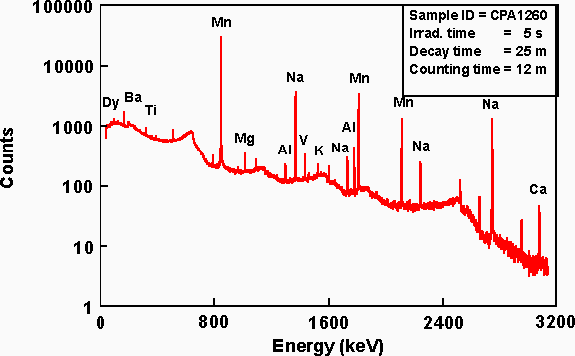
\includegraphics[width=\textwidth]{img/spect-1.png}
\caption{$\gamma$-Spektrum kurzlebiger El.\ einer Keramik-Probe, MURR.}
\end{figure}
\end{minipage}
\end{frame}

\begin{frame}{Schritt 4: $\gamma$-Spektroskopie}
\begin{figure}
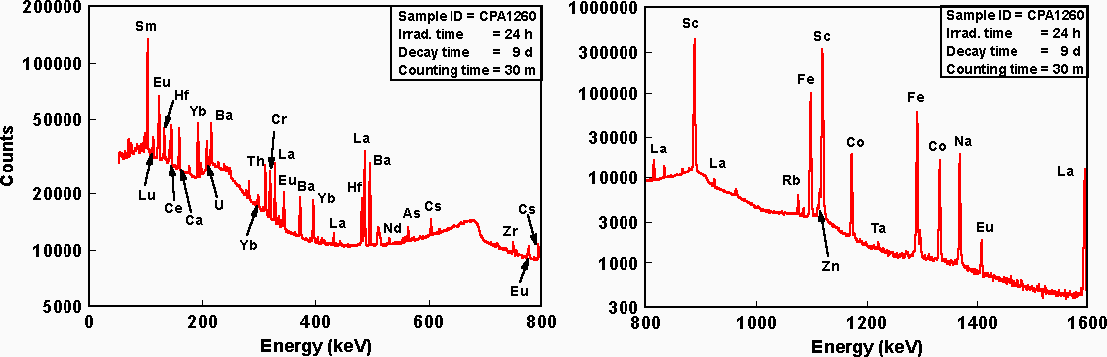
\includegraphics[width=\textwidth]{img/spect-2.png}
\caption{$\gamma$-Spektrum mittel- u.\ langlebiger El.\ einer Keramik-Probe, MURR.}
\end{figure}
\end{frame}

\subsection{Datenauswertung}

\begin{frame}{Schritt 5: Datenauswertung und Konzentrationsbestimmung}
\textbf{Wir haben gesehen:} Linien $\mapsto$ Elemente.
\begin{itemize}
\item 15--20 Linien aus Spektrum interessant
\item Mehrfachmessung einer Linie zu unterschiedlichen Zeiten
\item Korrekturen, z.\,B.\ bei Interferenzen und Überlappungen
\end{itemize}\medskip\pause

\textbf{Konzentrationsbestimmung:} Vergleich mit Referenzprobe!
\begin{itemize}
\item Jeweils Betrachtung eines Elements \textbf{in Probe und Referenz}:

\begin{center}
\alert{Intensitätsverhältnis $=$ Konzentrationsverhältnis}
\end{center}

(z.\,B.: Doppelte Linienstärke entspr.\ doppelter Konzentration)
\end{itemize}
\end{frame}

\begin{frame}{Schritt 5: Datenauswertung und Konzentrationsbestimmung}
\vspace*{-1em}
\Large Als Ergebnis erhalten wir den
\begin{huge}
\begin{center}
chemischen Fingerabdruck
\end{center}
\end{huge}
unserer Probe.
\end{frame}

\begin{frame}{Schritt 6: Mustervergleich}
\textbf{Gruppenbildung (\textit{Clustering)}:}
\begin{itemize}
\item Jede Probe $s$ ist ein \alert{Punkt} in einem $n$-dimensionalen Raum: \[s=(c_1,c_2,\dots,c_n)\] wobei $c_i$ die Konzentration des $i$-ten Elements in der Probe ist.\pause
\item Ähnlich zusammengesetzte Proben liegen in einer \alert{Punktwolke}.
\item Finden von Punktwolken durch statistische Verfahren am Computer

\alert{$\Rightarrow$ äquivalent zum Gruppieren der Proben!}
\end{itemize}
\end{frame}

\begin{frame}{Schritt 6: Mustervergleich}
\begin{minipage}{0.46\textwidth}\flushleft
Die Hyperräume werden durch \alert{Diskriminanzanalyse} auf eine zweidimensionale Fläche projiziert.\medskip	

Z.\,B.\ 3 Gruppen: Mittelpunkte der Wolken spannen Projektionsebene auf.\bigskip

\begin{figure}
\caption{Beispiel für Gruppierungen nach Diskriminanzanalyse.}
\end{figure}
\end{minipage}\hfill
\begin{minipage}{0.5\textwidth}
\begin{figure}
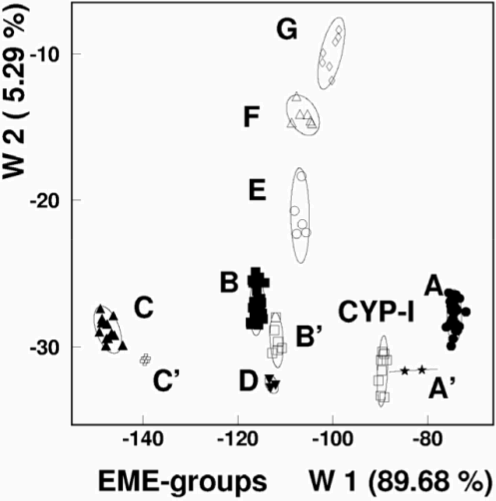
\includegraphics[width=.8\textwidth]{img/groups.png}
\end{figure}
\end{minipage}
\end{frame}

\section{Anwendungsbeispiel}

\begin{frame}<1>[label=aegina]{Beispiel: Keramik aus Attika}
\begin{minipage}{0.45\textwidth}\flushleft


\textbf{Ausgangssituation:} Zuordnungen von 224 mykenischen Keramiken aus Attika.\medskip\pause

\textbf{Problem:} Kein Referenzmaterial (z.\,B.\ Fehlbrände) vorhanden $\Rightarrow$ DB\medskip

\textbf{Ergebnis:} Kochkeramik aus Aegina,
sowie die meisten matt bemalten\medskip

Hochwertige Keramik fast komplett aus Argolis\medskip

\alert{$\Rightarrow$ Insg.\ 25\,\% importiert!}
\end{minipage}\hfill
\begin{minipage}{0.51\textwidth}
\begin{figure}
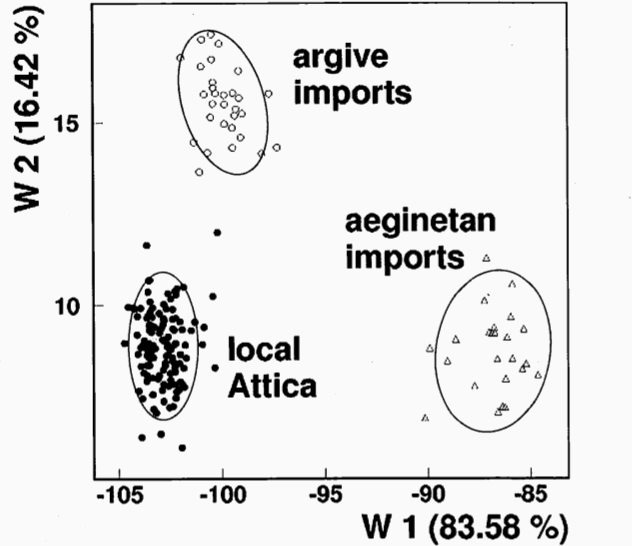
\includegraphics[width=.9\textwidth]{img/aegina.png}
\caption{Gruppierungen aus Attika, Aegina, Argolis. \cite{mommsen2003}}
\end{figure}
\end{minipage}
\end{frame}

{
\usebackgroundtemplate{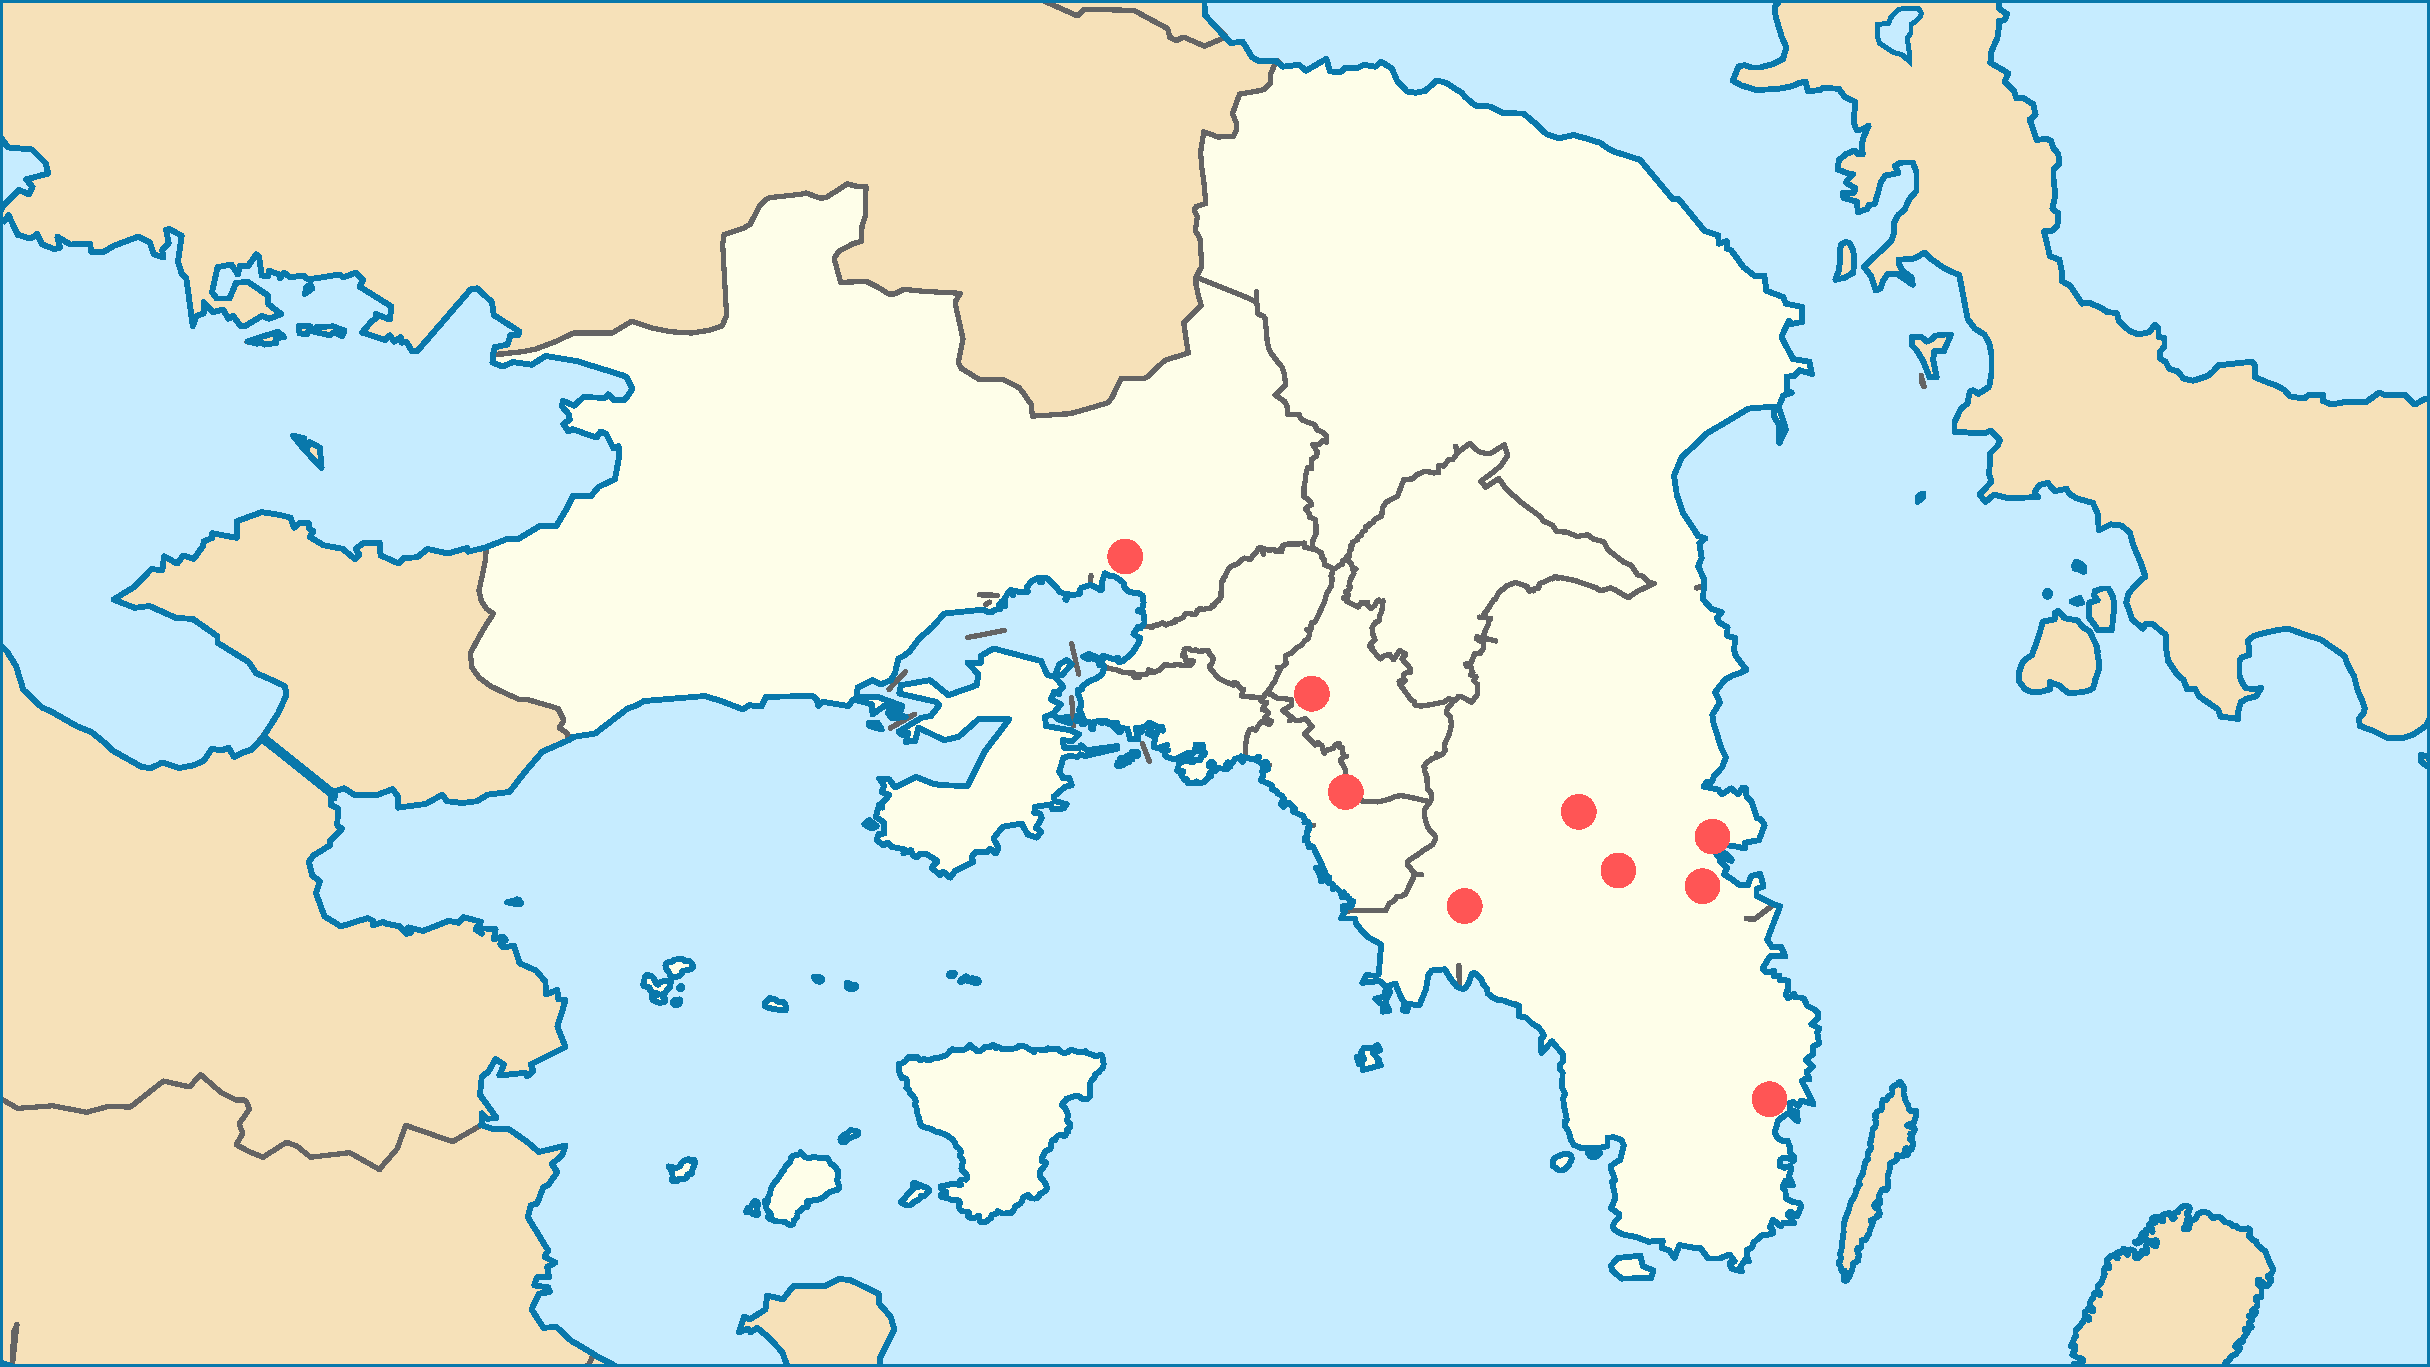
\includegraphics[width=\paperwidth]{img/attica.pdf}}
\begin{frame}[plain]
\end{frame}
}

\againframe<2->{aegina}

\begin{frame}{Beispiel: Keramik aus Attika}
\begin{figure}
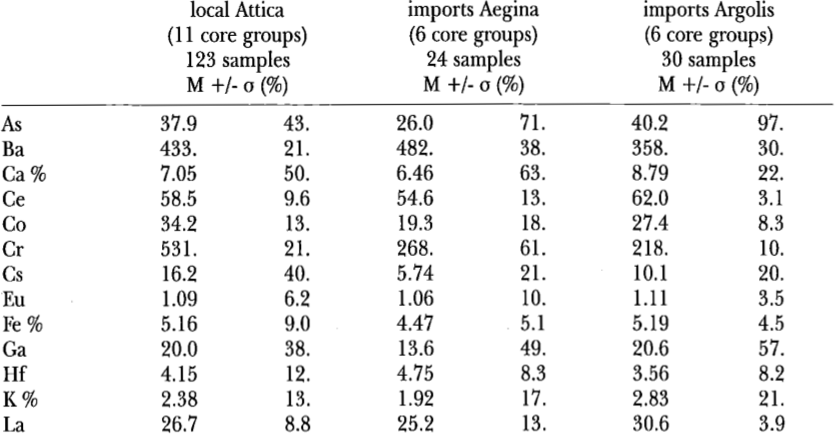
\includegraphics[width=.85\textwidth]{img/table-1.png}
\caption{Konzentrationswerte für Attika, Aegina, Argolis. \cite{mommsen2003}.}
\end{figure}
\end{frame}

\begin{frame}{Beispiel: Keramik aus Attika}
\begin{figure}
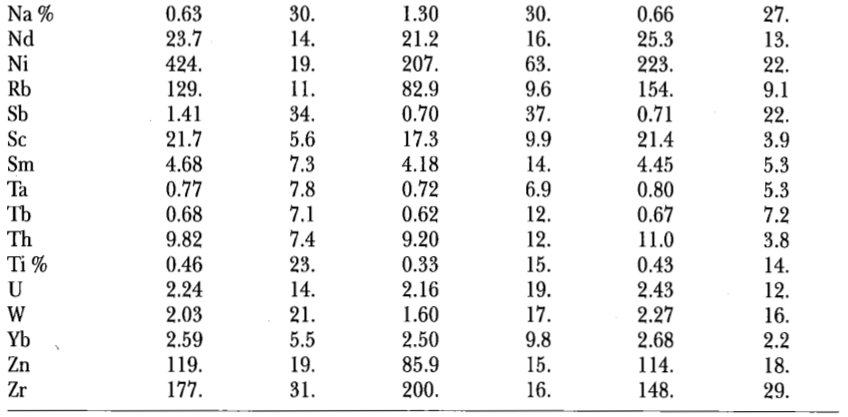
\includegraphics[width=.9\textwidth]{img/table-2.png}
\caption{Konzentrationswerte für Attika, Aegina, Argolis. \cite{mommsen2003}.}
\end{figure}
\end{frame}

\section{Einrichtungen}

\begin{frame}{MURR}
\begin{quote}
``The internationally recognized \textbf{University of Missouri Research Reactor (MURR)}, a 10-megawatt facility, is the \alert{most powerful} among the dozens of research reactors located on our nation’s university campuses. 

Even worldwide, few facilities can compare.''
\end{quote}
\vspace*{-2em}
\begin{flushright}
\href{www.murr.missouri.edu}{\texttt{www.murr.missouri.edu}}
\end{flushright}\bigskip
\end{frame}

\begin{frame}{TRIGA: Reaktoren für die Lehre}
\begin{figure}
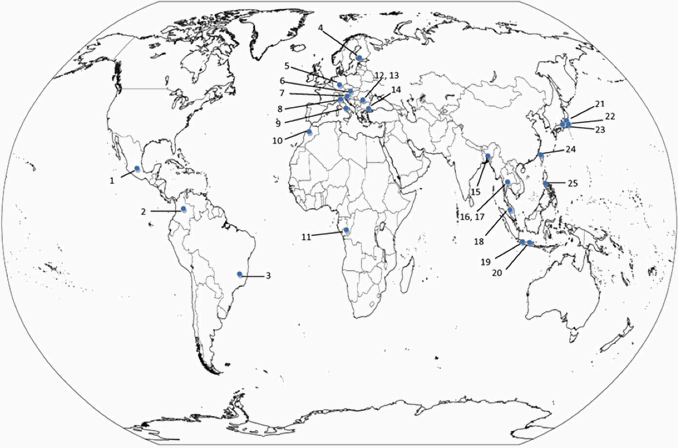
\includegraphics[height=.75\textheight]{img/triga.png}
\caption{Standorte v.\ TRIGA Reaktoren außerhalb d.\ USA.}
\end{figure}
\end{frame}

\begin{frame}{Kosten}
\begin{quote}
``[\dots] we have a multi-element survey for \alert{\$\,495 per sample}. [\dots] This test requires approximately \alert{6 weeks} and the error is approximately 20\,\%.''
\end{quote}
\vspace*{-2em}
\begin{flushright}
-- General Activation Analysis, Inc., CA
\end{flushright}\bigskip

\href{http://www.tnw.tudelft.nl/en/cooperation/facilities/reactor-instituut-delft/services/inaa/pricelist/}{Delft University of Technology}
\end{frame}

\section{Ausblick}

\begin{frame}{Ausblick}
Schlecht: Forschungsreaktoren sind weltweit \alert{stark begrenzt} und \alert{teuer}.\pause

\begin{center}
\Large$\Rightarrow$ Bleibt die Daseinsberechtigung von NAA?
\end{center}
\end{frame}

\begin{frame}{Ausblick}
\begin{minipage}[t]{0.48\textwidth}\flushleft
\textbf{JA}, denn NAA kann\ \dots\pause
\begin{itemize}
\item \alert{viele} Elemente \dots\pause
\item in \alert{mehreren Proben} \dots\pause
\item \alert{gleichzeitig} \dots\pause
\item und vollkommen \alert{automatisch} \dots\pause
\item mit \alert{hoher Sensitivität} messen!
\end{itemize}
\end{minipage}\pause
\begin{minipage}[t]{0.48\textwidth}
Es braucht dazu \glqq lediglich\grqq\ \dots
\begin{itemize}
\item eine \alert{geringe} Probenmenge

(ca.\ 80\,mg)\pause
\item einen Atomreaktor + Uran\pause
\item Geld\pause
\item und massig \alert{Zeit} ($>4$ Wochen) bis zum Ergebnis.
\end{itemize}
\end{minipage}
\end{frame}

\begin{frame}{Literatur}
\nocite{*}

\printbibliography[heading=none]
\end{frame}

\maketitle

\end{document}